\section{Обменяться зашифрованными сообщениями с другим пользователем gpg}

Для демонстрации передачи сообщений зашифрованных с помощью gpg был получен, импортирован и подписан сертификат другого пользователя 
gpg. Для подтверждения этого рассмотрим вывод утилиты gpg, запущенной с опцией \src{--list-keys}, представленный в листинге 
\ref{lst:keys-list}. Испортированный ключ соответствует пользователю \src{Sergey Klimov (Lab3) <ksa1993@yandex.ru>}.

\begin{listing}[H]
    \inputminted{console}{resources/09_keys_list}
    \caption{Вывод утилиты gpg при вызове с опцией \src{--list-keys}}
    \label{lst:keys-list}
\end{listing}

Для шифрования и подписи некоторого файла необходимо вызвать утилиту gpg с опциями \src{--sign} и \src{--encrypt}, а также 
с помощью опций \src{--local-user} и \src{--recipient} указать идентификатор сертификатов отправителя и получателя соответственно.
Пример вывода утилиты при шифровании файла указан в листинге \ref{lst:encrypt-file}. При этом, после вызова приведенной команды
будет создан greeting.txt.gpg, содержащий зашифрованные данные и электронную цифвровую подпись.

\begin{listing}[H]
    \inputminted{console}{resources/10_encrypt_file}
    \caption{Вывод утилиты gpg при вызове с опциями \src{--encrypt} и \src{--sign}}
    \label{lst:encrypt-file}
\end{listing}

Пересылка файла и его рассшифровка получателем прошли успешно.

Описанная выше операция по пересылке шифрованного сообщения была также в точности повторена со сменой ролей получателя и отправителя.
От другого пользователя gpg был получен зашифрованный файл pic.jpg.gpg, который был расшифрован с помощью опции \src{--decrypt} 
утилиты gpg, как показано в листинге \ref{lst:decrypt-file}. Расшифрованный файл представлен на рисунке \ref{fig:decryption-result}.

\begin{listing}[H]
    \inputminted{console}{resources/11_decrypt_file}
    \caption{Вывод утилиты gpg при вызове с опциями \src{--decrypt}}
    \label{lst:encrypt-file}
\end{listing}

\begin{figure}[H]
    \centering
    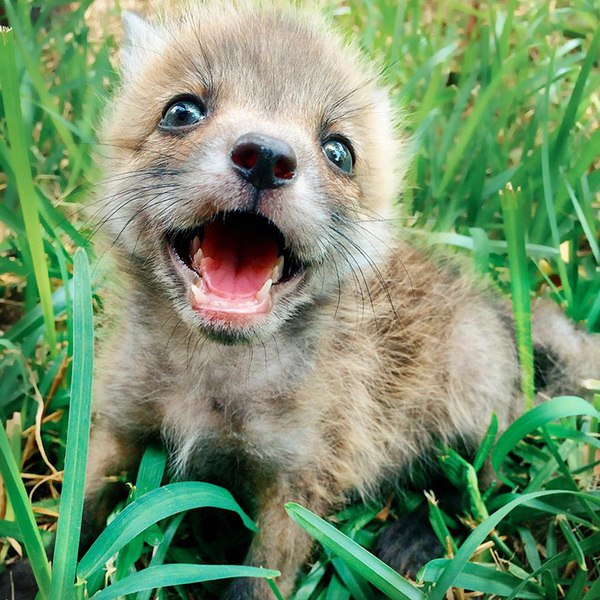
\includegraphics[width=18cm]{resources/12_decryption_result.jpg}
    \caption{Результат расшифровки сообщения}
    \label{fig:decryption-result}
\end{figure}